\documentclass{standalone}
\usepackage{hsbcommon}
\makeatletter\AtBeginDocument{\@buildstepset{1,2,3,4,5}}\makeatother
\begin{document}
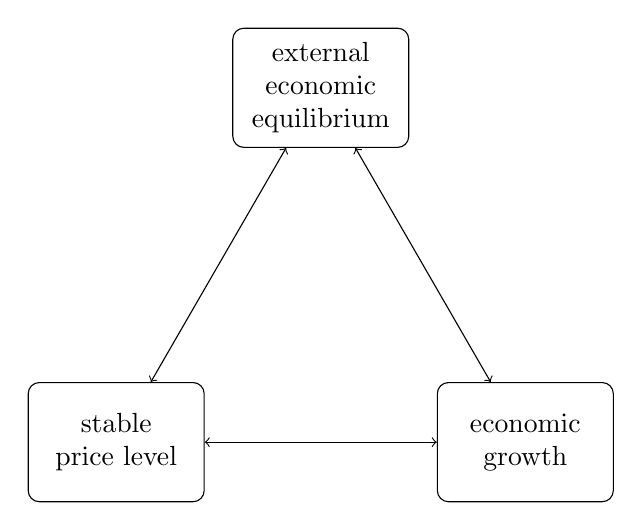
\begin{tikzpicture}[rotate=90]
    \tikzset{
        goal/.style={
            draw,
            text width=2cm,
            minimum height=10ex,
            align=center,
            rounded corners
        }
    }
    \foreach [count=\i] \myziel in 
    {%
    stable price level,
    economic growth,
    external economic equilibrium%
    }
    {
        \node[goal] (N\i) at (120*\i:3) {\myziel};
    }
    \draw[<->] (N1) -- (N2);
    \draw[<->] (N2) -- (N3);
    \draw[<->] (N3) -- (N1);


    

    
\end{tikzpicture}
\end{document}
